\documentclass{article}
\usepackage{color,soul}
\usepackage{graphicx}

\graphicspath{ {./images/} }

% Colors
\definecolor{blu}{rgb}{0,0,1}
\def\blu#1{{\color{blu}#1}}
\definecolor{gre}{rgb}{0,.5,0}
\def\gre#1{{\color{gre}#1}}
\definecolor{red}{rgb}{1,0,0}
\def\red#1{{\color{red}#1}}
\definecolor{lblu}{RGB}{10,213,216}
\def\lblu#1{{\color{lblu}#1}}

\def\image#1#2{{\includegraphics[scale=#2]{#1}}}
\def\html#1{{\textless#1\textgreater ... \textless/#1\textgreater}}

%Template
%\definecolor{x}{rgb}{0,0,0}
%\def\x#1{\color{x}#1}
\setul{0.5ex}{0.3ex}
\setulcolor{red}
 
\def\norm#1{\|#1\|}

% LaTeX
\def\items#1{\begin{itemize}#1\end{itemize}}
\def\enum#1{\begin{enumerate}#1\end{enumerate}}


\begin{document}

\title{Website Development Notes}
\author{Muhammad Ali}
\date{}
\maketitle

\section{HTML notes}
Consider the \html{header} tag which is usually used to identify content that precedes the primary content of the web page and often includes branding, navigation elements, search forms, and similar content.\newline \newline
\textbf{\html{nav}}: defines a set of navigation links usually for major block of navigation links.


\section{codeacademy: CSS}
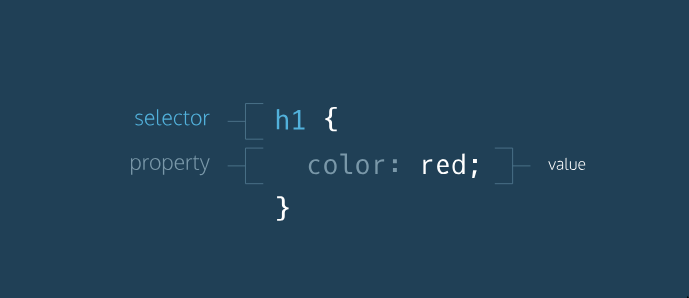
\includegraphics[scale=0.25]{css-outline.png}
\subsection{The box model}
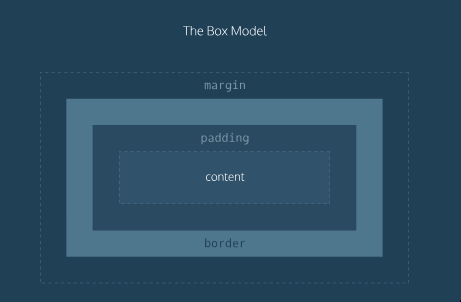
\includegraphics[scale=0.5]{box-model.png}

Content: includes text and other media \newline \newline
padding: \textit{as it looks like} \newline \newline
border: outline of an HTML page element. \textit{picture frame that contains the element}
use like \newline
\textbf{p \{ border: 2px [solid, dotted, dashed] [black, blue ...]\}} \newline \newline
margin: space b/w HTML page element and \textbf{next nearest element}. \newline
Also, doing something like \textit{p \{margin: 20px\}} will create spacings on each side of an element.\newline
You can do \textbf{margin-top, margin-bottom, margin-left, margin-right.}\newline \newline



\subsection{Block vs Inline Elements}
Allows to control the boundaries and space for individual HTML elements. It determines how HTML elements move around in the page.
\newline
\image{block-inline.png}{0.4}
\newline
\underline{These are properties for the css selector}\newline \newline
\ul{display:} [none, inline, block, inline-block]
\enum{
\item{\textbf{block:} HTML heading, paragraph, unordered list}
\item{\textbf{inline:} HTML image and anchor elements}
}
\ul{position:} [static, relative, fixed, absolute, sticky]
\enum{
\item{\textbf{static:} always positioned according to normal flow of page.}
\item{\textbf{relative:} Setting top, right bottom, and left properties of a "relative" positioned element will adjust it away from its normal position.\newline \image{relative.png}{0.3}}
\item{\textbf{fixed:} Just keeps some HTML element in the same place even when you're scrolling. You can use \textbf{top, bottom, right, left} to position it.\newline \image{fixed.png}{0.3}}
\item{\textbf{absolute:} positioned relative to the nearest positioned ancestor (instead of viewport like fixed)\newline \image{absolute.png}{0.3}}
\item{\textbf{sticky:} toggles between relative and fixed depending on the scroll position. Basically just follows you arround.\image{sticky.png}{0.3}}
}
\subsection{Using Float and Flex}
\textbf{Float}\newline
The float property is used for positioning and formatting content. Supports \textbf{left, right, none, and inherit}\newline
\image{float.png}{0.25}\newline
\textbf{Flex}\newline
\textbf{display: flex;}: Makes a flex container that makes the display flexible.\newline
\ul{Flex container properties}
\enum{
\item{flex-direction: properly defines which direction the container wants to stack the flex items with values \textbf{row, row-reverse, column, column-reverse, initial, inherit.}}
\item{flex-wrap: specifies whether the flex items should wrap or not with values \textbf{nowrap, wrap, wrap-reverse, initial, inherit}}
\item{flex-flow: property is short-hand for flex-direction and flex-wrap with values \textbf{flex-direction, flex-wrap, initial, inherit.}}
\item{justify-content: aligns the flex container's items when the items don't use all available space on the horizontal axis with values \textbf{flex-start, flex-end, center, space-between, space-around, initial, inherit.} Note: flex-start and -end position the items at start and end of container}
\item{align-items: Specifies the default alignment for items inside the container with values \textbf{stretch, center, flex-start, flex-end, baseline, initial, inherit.}}
\item{align-content: modifies the behavior of the flex-wrap property. Similar to align-items but aligns flex lines instead of flex itemswith values \textbf{stretch, center, flex-start, flex-end, space-between, space-around, initial, inherit.}}
}

\subsection{Bootstrap}
\image{bootstrap.png}{0.35}\newline \newline
This sizes css elements in a specified grid pattern and allows for you to have more dynamic webpages with the ."..." referring to class elements to include in the html elements.
\end{document}


